\documentclass{article}
\usepackage[utf8]{inputenc}
\usepackage{graphicx}
\usepackage[paper=a4paper,left=3cm, right=3cm, top=2cm]{geometry}
\usepackage{blindtext}
\usepackage{multicol}
\usepackage{pgfplots}
\usepackage{float}
\usepackage{biblatex} %Imports biblatex package
\usepackage{amsmath}
\addbibresource{main.bib} %Import the bibliography file
\usepackage{array}
\usepackage{caption}
\usepackage{subcaption}

 
\pgfplotsset{compat = newest}

\title{\textbf{Nuclear medicine imaging of neuroendocrine tumours}}
\author{Prachi Dewangan\\
\textit{Department of Biomedical Engineering} \\ National Institute of Technology, Raipur \\ Email: prachidewangan2001@gmail.com\\}
\date{}

\begin{document}
\maketitle
\begin{abstract}\textbf{In nuclear medicine, various tracers have been proposed to visualise neuroendocrine tumours; the majority are based on certain absorption mechanisms, while others are atypical. Radiolabeled metaiodobenzylguanidine (123I or 131I-MIBG) are two of the most important gamma-emitting tracers "It's worth mentioning in-pentetreotide. Good results can be obtained, in particular, with ' "In-pentetreotide scanning, which detects more than 70\% of all neuroendocrine tumours and has a diagnostic sensitivity superior to that of conventional radiological imaging in some indications, such as GEP tumours, has a diagnostic sensitivity superior to that of conventional radiological imaging. At the moment, radiolabelled monoclonal antibodies are primarily of historical relevance, but a variety of novel peptides offer intriguing issues in areas that are now being investigated. Positron emission tomography (PET) is a successful cancer detection method that has recently showed a high diagnostic value across a wide range of tumour types. PET using 18F-deoxyglucose (FDG) has also been used to identify neuroendocrine tumours. Even though 18F-FDG has been widely used in cancer, it has yet to show a significant absorption in well-differentiated neuroendocrine tissues. Other positron emitter tracers, on the other hand, appear to be more promising. Carcinoids have showed an enhanced absorption of the serotonin precursor 5-hydroxytryptophan (5-HTP) labelled with "C." This selective uptake appears to enable for the detection of more lesions with PET than with CT or octreotide scintigraphy, according to some clinical evidence. "C L-DOPA," a PET radiopharmaceutical in development, appears to be beneficial in imaging endocrine pancreatic tumours. The potential of several nuclear medicine techniques in the diagnosis of neuroendocrine tumours is summarised in this review, which also emphasises nuclear medicine's renewed role in the management of this disease. This selective uptake appears to enable for the detection of more lesions with PET than with CT or octreotide scintigraphy, according to some clinical evidence. "C L-DOPA," a PET radiopharmaceutical in development, appears to be beneficial in imaging endocrine pancreatic tumours. The potential of several nuclear medicine techniques in the diagnosis of neuroendocrine tumours is summarised in this review, which also emphasises nuclear medicine's renewed role in the management of this disease.
 } \\ \\
    
\end{abstract}

\begin{multicols}{2}

\section{Introduction}

Low incidence, low proliferation rate, and sometimes hypersecretion of biologically active chemicals are all characteristics that separate neuroendocrine tumours from other cancers. Because of the presence of unique secretory products and cytoplasmic proteins, they have a distinct histological pattern. These tumours have been the subject of research for the past 20 years, with the goal of better biological classification and the development of new management techniques. As a result, tremendous progress has been made in both diagnosis and therapy\cite{rindi2000introduction}.\\ \\
In terms of imaging procedures, advances in computed tomography (CT), magnetic resonance (MR), ultrasonography (US), intraoperative ultrasonography, angiography, and nuclear medicine have substantially aided tumour evaluation and, in general, led to the earlier detection of tiny tumour masses. Because many techniques have been developed in recent years, based on several different radiopharmaceuticals, and these new techniques have successfully been used to visualise neuroendocrine tumours, nuclear medicine has become increasingly involved in this topic. This is due to the different metabolic pathways and features of neuroendocrine tissue. Despite the fact that neuroendocrine tumours are rather uncommon, nuclear medicine professionals are frequently faced with the diagnosis of neuroendocrine lesions in their daily practise. Only the most relevant approaches in present clinical practise will be discussed in this review, as well as future views arising from ongoing experimental data\cite{capella1995revised}.

\section{Radiopharmaceuticals for neuroendocrine tumours imaging }
The radiopharmaceuticals used to visualise neuroendocrine tumours are chosen based on different metabolic pathways. In nuclear medicine, various tracers have been proposed; some are based on specific absorption mechanisms, while others are non-specific probes. It is important to note that, even if a specific absorption mechanism exists, it is not unique to a certain tumour type, as neuroendocrine cells are found throughout the body. Neuroendocrine cells, in reality, form small organs, separate cell clusters inside other tissues, or a network of cells scattered across the lungs, stomach, thymus, and thyroid\cite{estrozi2011neuroendocrine}. This is why each tracer can be utilised for a variety of clinical indications. Only the most important tracers will be considered in this review: some are currently in clinical use, such as metaiodobenzylguanidine (MIBG) and pentetreotide; others are of potential interest, such as positron emitters radiopharmaceuticals, VIP, and several new somatostatin analogues; others have historical value, such as radiolabelled monoclonal antibodies; and others will be phased out, such as 99mTc (V)\cite{ahmed2020gastrointestinal}. 


\subsection{Metaiodobenzylguanidine (MIBG)}
MIBG is made up of a benzyl group from bretylium and a guanidine group from guanithidine. In the early 1980s, radiolabelled MIBG was created to visualise disorders of the adrenal medulla. It is structurally similar to norepinephrine. It is taken up in the cell membrane of sympathomedullary tissues via an active, sodium- and energy-dependent (Type 1) amine absorption mechanism. It is carried into the intracellular catecholamine storage vesicles once it reaches the cytoplasm. MIBG is able to reach neuroendocrine circuits as a result of this absorption mechanism. The average component that allows for high selective uptake and imaging is the prolonged storage within the vesicles. Both 131I and I23I can be used to label MIBG. Injectable activity in adults ranges from 18.5 to 37 MBq for 13II-MIBG and 185 to 370 MBq for 123I-MIBG\cite{carvao2021neuroendocrine}. The 123I-labeled agent is the radiopharmaceutical of choice, according to theoretical considerations and clinical experience. It produces higher-quality images, has greater photon detection, and is more sensitive. To do single photon emission thomography, these properties are required (SPECT). Nonetheless, owing of its lower costs, availability, extended half-life, and ability to acquire delayed scans, I31I-MIBG is still frequently used for most regular applications. \\ \\
Even though there is some overlap in the types of neoplasms that can be detected with radiolabelled MIBG and in-pentetreotide, most studies imply that the indications may differ depending on the kind of tumour and clinical situation. MIBG scintigraphy, in our perspective, is currently the first-line treatment for functional phaeochromocytomas, paragangliomas, and neuroblastomas. Other neuroendocrine tumours, such as carcinoids, medullary thyroid carcinomas, and nonfunctioning paragangliomas, benefit from it\cite{board2002pancreatic}.

\section{DTPA-D-Phe-octreotide (pentetreotide)}
Somatostatin (SST) is a tiny multifunctional ciclic peptide produced by neuroendocrine and other cells found in a variety of organs and regions. Many neuroendocrin-derived cells and tumours have been found to have SST receptors (sstr). Molecular research revealed that there are five different types of somatostatin receptors, each with a different tissue distribution. Sstrl, sstr2 (with two splice variants, sstr2A and sstr2B), sstr3, sstr4, and sstr5 have been cloned and given cronological names. SST is not an appropriate tracer for imaging since it has a short half-life (1-3 minutes) and produces rebound hypersecretion upon withdrawal\cite{oberg2000state}. Octreotide-acetate was the first synthetic analogue created; the key limitations were the radiopharmaceutical's laborious labelling, limited availability, expensive cost, and high intestinal radioactivity. As a result, a novel tracer called DTPA-octreotide was created by combining ethilenetriamine-penta-acetic acid (DTPA) with octreotide (Pentetreotide). This tracer was first labelled with I23I and then with '"in.'"in-labeled pentetreotide binds to sstr2 exclusively. Because of its ability to bind to sstr2, which is found in many cellular membranes of neuroendocrine tumours, clinical trials have clearly proven that this receptor radiopharmaceutical is efficient in diagnosing and staging tumours and their metastases\cite{bajetta2000new}. Despite research efforts to generate more precise radioligands, "'in-pentetreotide" remains the radiopharmaceutical of choice for imaging neuroendocrine tumours at this time.\\ \\
In adults, 110-220 MBq of "'in-pentetreotide is injected; roughly 80\% of i.v. given radiolabelled "'in-pentetreotide is removed through the urine system. Even though somatostatin receptors are found in a wide range of tumours, "The principal indication for in-pentetreotide is as a diagnostic agent for the location of primary sites and metastases in GEP-tumours (carcinoids, islet cell tumours, gastrinomas, insulinomas, glucagonomas, VIPomas). Many other tumours have been seen using this technique "Somatostatin receptors are found in a high number of cancers, including medullary thyroid carcinoma (MTC), small-cell lung cancer (SCLC), phaeochromocytoma, pituitary tumours, and CNS tumours. Somatostatin receptors are also found in breast carcinoma and renal tumours. However, the effectiveness of niIn-labeled pentetreotide scanning in patients with these tumours has yet to be proven.

\section{Clinical applications of nuclear medicine imaging}

\subsection{Gastroenteropancreatic tumours (GEP)}
Neuroendocrine GEP tumours are a group of neoplasms that arise from neuroendocrine cells found in the epitelium of the gastro-intestinal tract (carcinoids, islet cell tumours, gastrinomas, insulinomas, glucagonomas, VIPomas). The research and present experience at our Institute indicate that "in-pentetreotide scintigraphy is particularly effective for patients with small-bowel carcinoids that are difficult to localise using conventional methods." Because SPECT imaging can detect more lesions than planar imaging or radiological treatments, it is required in cases of clinical uncertainty. Carcinoids can be seen regardless of tumour location or hormonal hypersecretion, and whole-body scanning can reveal distant metastases. SST receptor imaging may be particularly beneficial for localising a tumour site when surgery is scheduled because of its great sensitivity.
Islet cell tumours emerge from endocrine pancreatic cells and are termed after the secreted hormone they produce (gastrinoma, VIPoma, Insuloma); 15\% of these tumours are not linked to hypersecretion syndrome. The most common type of islet cell tumour is gastrinoma, which accounts for 10\% of all GEP tumours. Somatostatin receptors are found in high quantities in most malignant islet cell carcinomas, according to clinical evidence. The sensitivity of "in-pentetreotide scintigraphy" has been reported to range from 70\% to 90\%, with some of the variance likely attributable to faulty scanning procedures and failure to do SPECT investigations.
Islet cell tumours emerge from endocrine pancreatic cells and are termed after the secreted hormone they produce (gastrinoma, VIPoma, Insuloma); 15\% of these tumours are not linked to hypersecretion syndrome. The most common type of islet cell tumour is gastrinoma, which accounts for 10\% of all GEP tumours. Somatostatin receptors are found in high quantities in most malignant islet cell carcinomas, according to clinical evidence (Figures 2a and 2b). The sensitivity of "in-pentetreotide scintigraphy" has been reported to range from 70\% to 90\%, with some of the variance likely attributable to faulty scanning procedures and failure to do SPECT investigations.

\begin{figure}[H]
    \centering
    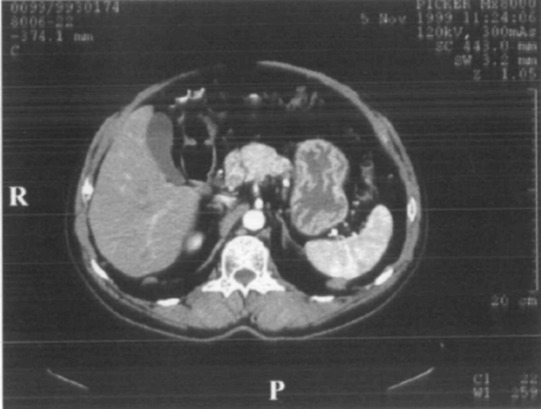
\includegraphics[width=6cm]{images/WhatsApp Image 2022-04-08 at 5.03.03 PM.jpeg}
    \caption{CT scan of the pancreatic lesion demonstrated by the whole body scan with 111In-pentetreotide. Morphologic imaging clearly defines the topographic location of the tumour and the relationships with the surrounding organs.}
    \label{fig:1}
\end{figure}

\subsection{Phaeochromocytoma and paraganglioma}

MIBG radiolabelled with I23I and 131I is the most extensively used radipharmaceutical for the diagnosis of phaeochromocytoma, with a total sensitivity of roughly 90\%. MIBG is helpful in identifying and locating intra-adrenal (phaeochromocytomas) and extra-adrenal (paragangliomas) paragangliomas. The MIBG whole body scan can be used to identify the degree of the disease (staging) and to diagnose relapses throughout the postoperative period. The use of MIBG has the added benefit of allowing patients to be selected for subsequent radiometabolic therapy depending on MIBG uptake into cancer cells. 
The sensitivity of SST scintigraphy for phaeochromocytoma identification appears to be better or comparable; nevertheless, the number of patients studied so far is insufficient to draw any conclusions. The outcome is partly dependent on the tumour site, as it is well known that due to its high renal activity, inpentetreotide makes it difficult to visualise adrenal tumours.
The 111In-pentetreotide whole body scan has proven to be quite accurate for paraganglioma tumours, revealing several unexpected additional paraganglioma localizations not found with other conventional scans. Even though MIBG imaging has a high specificity, clinical evidence shows that SST scintigraphy has a higher sensitivity for paraganglioma than any other nuclear medicine test or radiological procedure (CT, MR, US). One of the key advantages of SST scintigraphy in this regard is that it provides information on probable tumour localizations throughout the body. This supports some authors' recommendations that luIn-pentetreotide scintigraphy be used as the first diagnostic test in patients with paraganglioma, followed by CT scanning, MR, or US of the anomalies detected.

\subsection{Medullary carcinoma of the thyroid gland (MTC)}

Many radiopharmaceuticals (including the lyphofilic cation 99mTc-Sesta-MIBI) have been offered for scintigraphic visualisation of this tumour, and no experience has been allowed to have a decisive and univocal effect. Clinical tests and monitoring of changes in serum levels of calcitonin and/or CEA are currently used to follow up on individuals who have had a complete thyroidectomy. Increased postsurgical calcitonin and/or CEA levels suggest chronic disease, but a progressive increase after normalisation indicates relapse; the clinical difficulty in this scenario is to detect cancer. Intra-operative venous catheterization is one of the most effective techniques. This allows us to pinpoint the mass-producing calcitonin with high sensitivity and specificity, but it is an invasive procedure that can only be conducted in a few centres. According to a recent study, scintigraphic detection of recurrent metastatic MTC using labelled anti-CEA monoclonal antibodies or "'In-pentetreotide appears to have a sensitivity that is superior to any other diagnostic modalities. When examining the cost-effectiveness of SST imaging in patients with MTC, however, the data show that receptor scintigraphy adds nothing to the information received from other types of imaging. To summarise, until now, the radiopharmaceutical that has been deemed the most effective and least expensive for detecting MTC has been 99mTc DMSA; nevertheless, its production for the market will be halted. MIBG scan has demonstrated minimal utility in the clinical management of MTC; the diagnostic performance of this tracer varies greatly depending on the author. MIBG uptake, on the other hand, may be high enough to allow radionuclide therapy. MIBG imaging should be used in this situation to assess such a therapeutic option\cite{kurtaran1999receptor}. 

\subsection{Lung tumours}
The sensitivity of 111In-pentetreotide scintigraphy in imaging small-cell lung cancer (SCLC) primary tumours ranges from 85 percent to 100 percent; the sensitivity in imaging known metastases appears to be lower. However, SST scintigraphy has discovered additional areas of disease in several trials, and this data can have a significant impact on cancer staging and treatment. Despite SST scintigraphy's varying sensitivity for distant metastases, which is likely owing to changes in the expression of SST receptors on metastatic lesions, clinical application of this technique can provide extra information in staging patients. It goes without saying that the discovery of unanticipated cerebral metastases or the upstaging of patients from limited to extensive disease (as determined by conventional imaging) may have an impact on patient care strategies. The use of mInpentetrotide scintigraphy in the staging of SCLC patients is still up for debate. However, considerable clinical data and evaluations derived from cost-effectiveness analyses appear to suggest that the cost increase relative to a standard work-up can be justified by the therapeutic outcomes.

\subsection{Neuroblastoma}
MIBG is still a particular radiopharmaceutical for neuroblastoma, since 123/I3II-MIBG scintigraphy provides a non-invasive method for diagnosing neuroblastoma in a child with a tumour mass of uncertain origin. Overall, 91.5 percent of neuroblastomas concentrate MIBG, making I23/131I-MIBG scintigraphy combined with urinary detection of catecholamine metabolites the most sensitive indications of neuroblastoma, according to a large series of 844 patients described in the international literature. Whole-body scintigraphy allows for the detection of metastases anywhere in the body, which is critical for disease staging and frequent stage upgrades; the number of lesions has a predictive value. I 2 3 / I 3 IT after treatment (surgery, chemotherapy, or radiotherapy). MIBG scintigraphy is commonly used as a functional marker of response, and its main advantage is the ability to examine alterations lesion-by-lesion. Because of the high concentration of I31I-MIBG in tumour masses, its low concentration in healthy tissues, and the comparatively long half-life of 13II-MIBG, therapy with high radiopharmaceutical activity is possible. 111In-pentetreotide scintigraphy has no clinical value at the moment, given the primary role that MIBG has played in the clinical therapy of neuroblastoma. SST receptor scintigraphy, on the other hand, is positive in roughly 90\% of neuroblastoma patients. Clinical research suggests that patients with neuroblastoma who have tumour tissues that express SST receptors in vitro have a better prognosis than those who do not. This research implies that the presence of SST receptors can be used to predict prognosis.

\subsection{Pituitary tumours}
In vitro, SST receptors were found in GH-producing pituitary adenomas. SST receptor positivity is found in the majority of individuals with pituitary adenomas, and different authors have reported positive scintigraphic results in patients with clinically non-functioning pituitary adenomas. The uptake of luIn-pentetreotide is higher in patients than in control subjects, as seen by scintigraphy, and the responses to medical treatment are related to scintigraphic uptake intensity. As a result, "in-pentetreotide scintigraphy" may be useful as a functional test for predicting and monitoring therapy response. The diagnostic accuracy, on the other hand, is weak, which limits its clinical applicability.

\subsection{Intraoperative diagnosis - radioguided surgery}

Radioguided surgery is based on the use of an intraoperative radiation detector that can identify and pinpoint cancer cells using a radiopharmaceutical that binds to tumours selectively. The high sensitivity of this technology is due to the fact that the detector probe can be put directly to the tissue, allowing for the detection of extremely small clusters of cancer cells. Sentinel node scintigraphy and intraoperative sentinel node identification is a typical example that has been successful in breast cancer and melanoma patients employing radiolabelled colloids trapped in metastatic lymph nodes. This application can also use radiopharmaceuticals used for neuroendocrine tumour imaging (radiolabelled monoclonal antibodies, 111In-pentetreotide, 99mTc-DMSA(V), 125I, and 13II-MIBG). Several studies have shown that intraoperative detection and/or radioguided surgery of neuroendocrine tumours can aid in determining the exact location of tumour tissue, attaining a complete resection of a tumour mass, finding residual tumour after incomplete resection, and screening for relapses. During laparotomic staging, this nuclear medicine method can be effective in identifying some concealed microscopic metastatic locations. Several fascinating reports on GEP tumours, medullary thyroid carcinoma, and neuroblastoma have been reported.

\subsection{Diagnostic application of positron emission tomography (PET)}

PET has shown considerable improvements for patient diagnosis and management in the last five years, particularly in oncology. The high sensitivity and resolution of this advanced technology, as well as the capacity to perform whole-body scans, the fact that PET provides functional images, and the ability to measure tracer uptake, are all reasons for PET's great success as a clinical tool. PET imaging is based on the properties of cancer tissue as a whole (proliferative activity, viability, other biological parameters). PET, in other words, produces metabolic images in addition to the morphological images produced by RX, US, CT, and MR. As a result, PET has the capacity to examine various tissue activities using a range of metabolic tracers. Unfortunately, the most extensively utilised PET radiopharmaceutical, 18F-FDG, fails to see tumours that are highly differentiated and have a low proliferation rate. Enhanced FDG absorption (indicating increased glucose metabolism) is exclusively seen in neuroendocrine tumours that lack SSTreceptors and have a strong proliferative activity. As a result, this examination reveals information that contradicts that obtained by ulIn-pentetreotide or I23/I31I-MIBG, both of which are associated to tissue differentiation. Other researchers have backed up this theory, confirming that the most clinically aggressive neuroendocrine tumours have a high FDG uptake\cite{mcewan1985radio}. In fact, FDG-PET appears to have a better sensitivity than SST receptor scintigraphy in these cancers with a bad prognosis. Of course, in patients with neuroendocrine tumours who have I8F-FDG uptake, FDG-PET can detect some metastatic lesions that aren't visible with other conventional imaging modalities. FDG-PET has been advocated by several authors as a diagnostic tool for medullary thyroid carcinomas, phaeochromocytomas, and paraganglioma staging and monitoring. The fact that 18F-FDG isn't a good tracer for neuroendocrine tissue prompted researchers at Uppsala University to develop various alternative positron emitter radiopharmaceuticals based on different precursors, such as 5-hydroxitriptophan (5HTP) and L-DOPA tagged with 11C\cite{short1967sympathetic}.\\ \\ 

In fact, FDG-PET appears to have a better sensitivity than SST receptor scintigraphy in these cancers with a bad prognosis. Of course, in patients with neuroendocrine tumours who have I8F-FDG uptake, FDG-PET can detect some metastatic lesions that aren't visible with other conventional imaging modalities. FDG-PET has been advocated by several authors as a diagnostic tool for medullary thyroid carcinomas, phaeochromocytomas, and paraganglioma staging and monitoring. The fact that 18F-FDG isn't a good tracer for neuroendocrine tissue prompted researchers at Uppsala University to develop various alternative positron emitter radiopharmaceuticals based on different precursors, such as 5-hydroxitriptophan (5HTP) and L-DOPA tagged with 11C.

\section{Conclusion}
A variety of tracers are currently available for imaging neuroendocrine tumours. The capacity to take in and store amines, the expressions of receptors on their surface, the improved glycolytic metabolism, and the capacity to take up some metabolic precursors are all biological mechanisms that characterise the biology of this particular neuroendocrine system. Several factors should be considered while selecting radiopharmaceuticals for use in clinical practise. The frequency of the presence of a certain pathway shared by the majority of endocrine cells is the first factor to evaluate. In this context, MIBG is an appropriate radipharmaceutical for tumours like phaeochromocytoma, which are characterised not only by amine absorption but also by the existence of specialised storage vesicles. Almost all neuroendocrine cells express SST receptors. As a result, ulIn-pentetreotide scintigraphy has demonstrated a high sensitivity for detecting both primary and metastatic tumour lesions. Somatostatin receptors, on the other hand, are expressed in varying degrees of strength; high levels are generally identified in GEP tumours, whereas lesser expression is found in other cancers (e.g.medullary thyroid tumours). All neuroendocrine tissues may display antigen structures, however in this situation, a constraint is the limited bioavailability of immunological detection probes, which have little clinical relevance in this setting. Because the metabolic activity of neuroendocrine tumour cells appears to be lower than that of normal cells, FDG-PET has not been used as widely as other oncological purposes. This is why FDG-PET positive is regarded an aggressiveness prognostic criterion, and FDGPET indications are confined to less-differentiated neuroendocrine tumours lacking SST receptors and with significant proliferative activity. Alternative positron emitter radiopharmaceuticals are being developed to investigate metabolic routes other than glucose. With 11C 5HTP and 11C L-DOPA, promising results have been obtained in this field. \\ \\
Based on these biological findings, 111In-pentetreotide and 123/I3II-MIBG remain the most often used and successful tracers for neuroendocrine tumour scintigraphy. Other criteria that might be considered for the selection of radiopharmaceuticals, in addition to uptake mechanisms, include dosimetry, cost-effectiveness, radioisotope availability, patient preparation, methodological considerations, and instrumentation facilities. We attempted to include the most important facts that, in our opinion, should be remembered for a practical routine in this overview.
\end{multicols}

\printbibliography

\end{document}
